\chapter{A GNN approach to the problem}
\label{chap:gnn}
So far we have experimented with various models trying to predict the Fock matrix as a whole. However, as has been seen in \autoref{chap:fock_matrix_predictions} this approach, which works on minimal basis sets, is not feasible for larger basis sets such as the 6-31G(2df,p) basis set. Recent advances using regression models have largely focused on separate models for each molecular species, which limits their applicability to constitutional isomers we are interested in. \parencite{ref:Hazra2024,ref:Shao2023}
We shall investigate the applicability of Graph Neural Networks (GNNs) to the problem of predicting the Fock or the density matrix. They have shown promising results in the field of quantum chemistry, especially for predicting molecular properties and structures. \parencite{ref:schnet2018}\\

The implementation of the GNN in this chapter is based on the \texttt{pytorch-geometric} framework \parencite{ref:PyTorchGeometric, ref:PyTorch_geom_paper}. 
\section{Input \& Output Matrices}
\label{sec:gnn_input_output_matrices}
Generally the input and the output of neural networks is fixed. We thus need to find a specific way to embed our input (overlap matrix) and output (Fock or density matrix) into a fixed structure. Given the nature of our problem, we can simply split our matrix representation into blocks representing the different atom sorts and their respective combinations. This yields three different types of matrix-blocks: 
\begin{itemize}
    \item \textbf{Self-blocks:} These blocks mix orbitals of the same atom type, e.g. $\text{\ch{O}}_0$ or $\text{\ch{H}}_1$\footnote{Subindices only enumerate elements and are not part of the chemical formula}. The self-blocks are diagonal blocks of the input and output matrices.
    \item \textbf{Homo-blocks:} These blocks mix only orbitals of the same atom type, e.g. $\text{\ch{H}}_1 - \text{\ch{H}}_2$.
    \item \textbf{Hetero-blocks:} These blocks mix orbitals of different atom sorts, e.g. $\text{\ch{O}}_0 - \text{\ch{H}}_2$.
\end{itemize}
Subsequently, we shall label self-blocks as node-blocks and homo- / hetero-blocks as interaction blocks interchangeably. 

A schematic depiction for the \ch{H2O} molecule using the 6-31G(2df,p) Basis is given in \autoref{fig:schematic_gnn_blocks}. Due to the symmetry of our input and output matrices we are only concerned with the upper triangular matrices for self-blocks and the homo- / hetero-blocks in the upper triangular part with respect to the full matrix. For the given example we thus have 351 entries for \ch{O} and 15 for \ch{H} self-blocks. Additionally, the \ch{H} homo-blocks yield 25 entries each and we obtain 130 values per \ch{O}-\ch{H} hetero-block. In total 666 entries suffice to reconstruct the full $36 \times 36$ matrix. 
\begin{figure}[H]
    \centering
    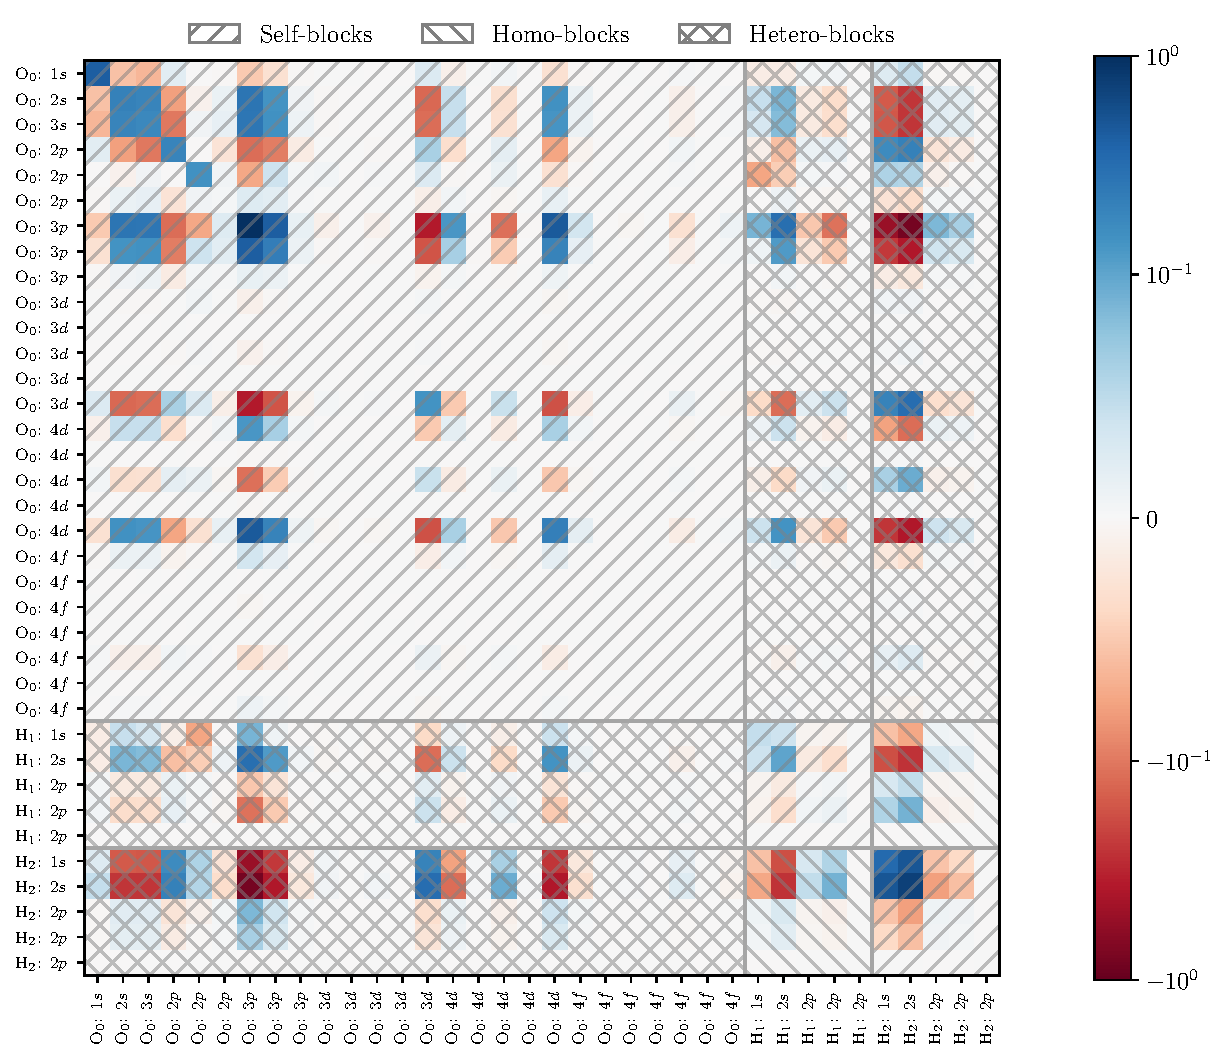
\includegraphics[width=\textwidth]{../fig/gnn/schematic_blocks.pdf}
    \caption[Matrix block regions of \ch{H2O}]{Converged density of \ch{H2O} with matrix block types indicated.}
    \label{fig:schematic_gnn_blocks}
\end{figure}
Evidently, the different block types vary widely in size. This needs to be addressed before feeding the data into the network. There are multiple ways of addressing this problem. A straightforward solution includes a simple zero pad to the maximum block size and subsequent masking. \TODO{Maybe cite Dominik here} Another approach is the compression or transformation to a fixed size latent space or some sort of pooling to reach the desired input dimension. In order to not loose relevant data we take yet another route and encode each block using separate encoders. Via this approach we mitigate the problem of different sized inputs as long as the basis set is fixed. For the example in \autoref{fig:schematic_gnn_blocks} we would thus have four differently sized encoders (two for the self-blocks and one for homo-/ and hetero-blocks respectively). These encoders will transfer the input features into a common hidden dimension to be used in the network. After the propagation through our GNN the decoder side will decode the output dimension of our network to the respective block dimensions from which the whole matrix can be reconstructed.
\section{Preprocessing}
\label{sec:gnn_preproc}
Before feeding our data into the network we must bring it into a suitable form for learning with the \texttt{pytorch-geometric} framework \parencite{ref:PyTorchGeometric, ref:PyTorch_geom_paper}. After introducing the design of our data objects and graph creation we discuss a way to tackle the problem's sensitivity to spatial rotation before closing out with normalization and dataset creation remarks. 
\subsection{Graph creation}
\label{subsec:gnn_graph_creation}
A graph representation of our data is required which will be populated using the paradigms described in \autoref{sec:gnn_input_output_matrices}. Nodes of our graph are essentially represented by embeddings of our overlap self-blocks. This leaves us with one node per atom in our molecule. To enable easier benchmarking and training processes the targets (Fock- or density matrix-self blocks) are also stored in our graph object. Nodes are connected by directed edges which are given by an embedding of the homo- / hetero-block regions under a given restriction. The restriction on edge formation may be given by a distance cutoff (e.g. \SI{3}{\angstrom}), but not necessarily limited to that method. In particular, for bonds involving high-angular-momentum orbitals, the highly directed radial extension of the electronic wavefunction should also lead to an edge between these respective nodes. Edge formation can thus be controlled by a threshold with regard to the maximum value or another metric e.g. a matrix norm for a given interaction interaction block. A tensor of indices is used to represent the directed edges between nodes identified with said index. Every bond is represented by two directed edges to support bidirectional data exchange between nodes.\\

Additionally, to the node and edge embeddings of our inputs and targets we store node atom-symbols and edge-symbols (e.g. \ch{C}-\ch{O}) to match encoder / decoder later on in our network. Furthermore, we store global index information for both node and interaction blocks to facilitate matrix reconstruction from our block representation. 

\subsection{Data Augmentation}
\label{subsec:gnn_data_augmentation}
The input (overlap) as well as output (Fock / density matrix) are quantities which are not generally invariant under rotations of our molecular system. In essence this means that we must find a way to learn differently rotated molecules and produce their respective Fock / density matrices to later deduce our initial density. While the idea of making the input invariant under rotation, by using a predetermined standard orientation, was initially considered, problems arise with this approach. Most prominently, defining a standard orientation for isomers / isomer-parts, such as \ch{C7H10O2} or submolecules thereof, is far from trivial. Even if such a standard orientation is defined, one has to consider an additional pre- and post-processing step to rotate the input into the standard orientation and the output back to the original orientation. \\
Contrary to this, the model can learn differently rotated inputs to generate the corresponding outputs. This is achieved by augmenting the dataset with different rotations of the same molecules / submolecules. Rotating the input coordinates using a rotation matrix $R$ is in principle rather straightforward. However, the corresponding overlap, density and Fock matrices also have to be transformed accordingly or recalculated. The later is computationally not feasible, hence we use the corresponding Wigner D-matrices to transform input and output matrices. 
The Wigner D-matrix is a unitary matrix with $2L + 1$ rows and columns, where $L$ is the angular momentum. For a given rotation $R$ the Matrix elements of overlap, density and Fock matrix transform according to:
\begin{equation}
    \label{eq:wigner_d_transform}
    O'_{ij} = \sum_{k,l} \mathcal{D}^{(L)}_{ik}(R) O_{kl} \mathcal{D}^{(L)*}_{lj}(R)
\end{equation}
Naturally, the transformation only acts on spatial orbitals with no rotational symmetry along the axis of rotation (i.e. $L \neq 0$). Given the blocks defined in \autoref{sec:gnn_input_output_matrices} $\mathcal{D}^{(L)}$ will only transform elements of the blocks with at least one orbital having $L \neq 0$. \\


Concretely, the input data is augmented by sampling a random rotation axis, using 3 normally distributed values to obtain an axis and a random rotation angle $\theta \in [0, 2\pi]$. Given this axis and angle, the corresponding transformations are performed to the overlap, density and Fock matrices to obtain augmented samples. New graphs are created using these transformed matrices as explained in the precious section and added to the dataset. \\
Due to grid spacing in DFT calculations small deviations ($\approx 0,1 \unit{\milli\hartree}$ in the Fock matrix) between the transformed matrices and newly calculated ones using the rotated atom coordinates occur. These deviations only slightly affect the accuracy of the reconstructed density (see \autoref{eq:density_reconstruction_from_fock}) and are not relevant during training, as we evaluate the model against the provided target. In other words, if the model predicts the density via the Fock matrix, we compare it to a reference density that was also reconstructed from the (transformed) Fock, not from a directly transformed density matrix.\\
%! Note that translating the molecule should change absolutely nothing about the Overlap or Fock matrix. 

\subsection{Normalization \& data split}
\label{subsec:gnn_normalization}
Means and standard deviations are calculated on a per block-type basis (e.g. for the \ch{O}-\ch{H} hetero-block) on all training data samples. This is done for the input (overlap matrix) and the output / targets (Fock or density matrix).\\
It should be noted that the inclusion of data augmentation samples does not change these values besides machine precision errors. The normalization is then performed by subtracting the mean and dividing by the standard deviation for each block-type. To avoid numerical instabilities, especially for very sparse blocks (std. dev $\rightarrow 0$), a value of $10^{-6}$ is used should the standard deviation fall bellow this value for a given block. \\

The dataset is ultimately split into training, validation, and test sets, typically following a ratio of 80\% / 10\% / 10\%, where 100\% refers to the number of original (non-augmented) samples.

When applying a data augmentation factor of $1.5$, meaning that 50\% more samples are generated synthetically, the training set is extended to contain 120\% of the original data, while the validation and test sets remain unchanged at 10\% each. This ensures that evaluation is performed exclusively on the original, unaltered data and avoids any data leakage through augmented samples. To ensure comparability of benchmarks in \autoref{chap:application} the \texttt{scf\_guess\_datasets} package was used to obtain samples \parencite{ref:milacher_scf_guess_datasets}.

\section{GNN Design}
\label{sec:gnn_design}
The basic design of the GNN is given by 

\begin{figure}[H]
    \centering
    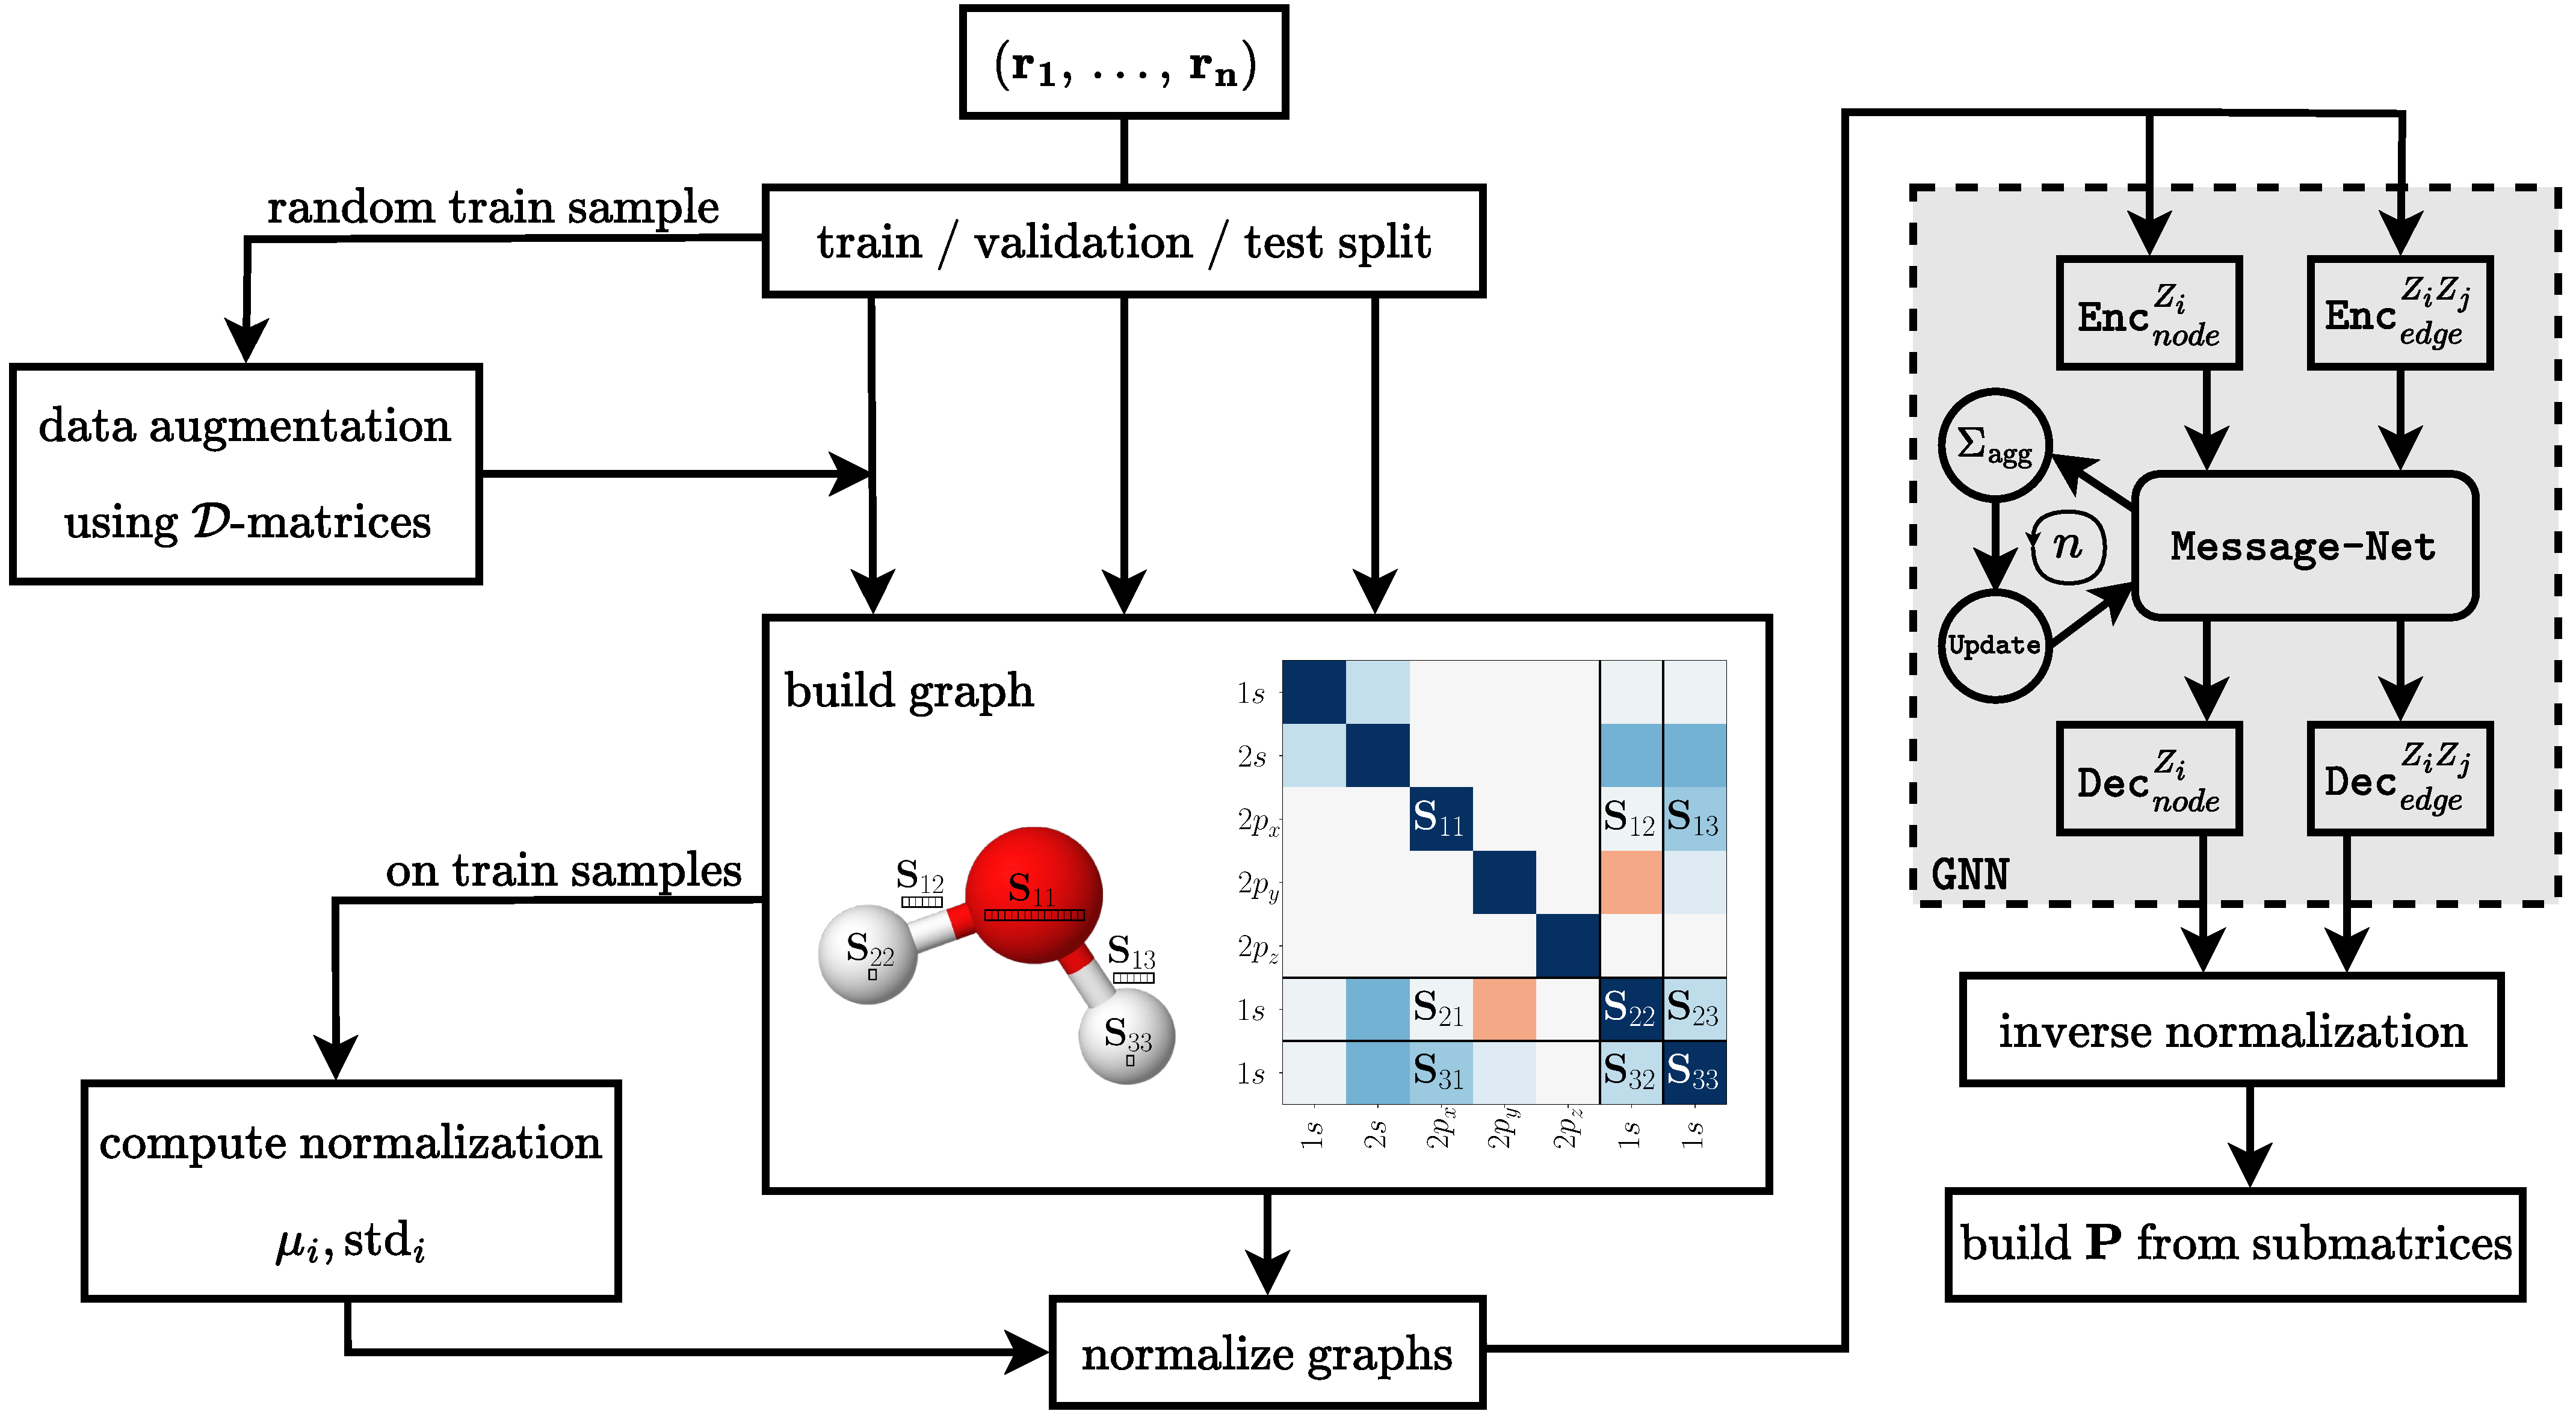
\includegraphics[width=\textwidth]{../fig/gnn/GNN_design.pdf}
    \caption[GNN design]{GNN design}
    \label{fig:gnn_design}
\end{figure}

% \TODO{Nice representation of orbitals on mols - maybe PyMol plot + some overlap matrix blocks}
\section{Training}
\label{sec:gnn_training}

The GNN will be trained using various hyperparameters and configurations in the following. All runs will be tested on QM9 \ch{C7H10O2} molecules which were simulated as reference using the B3LYP functional and the 6-31G(2df,p) basis set. If not stated otherwise, the train / validation / test split is set to 80\% / 10\% / 10\%.\\
\TODO{}

\subsection{Initial Training}
\label{subsec:gnn_initial_training}
To gauge the performance of the GNN on our problem, we will start with a sample using 500 molecules (400 / 50 / 50 for train / validation / test) randomly sampled from the 6095 isomers of \ch{C7H10O2}. 

Average iterations own: 11.42 +- 0.77, minao 11.00 +- 0.56

\TODO{}

% Meta: 
% \begin{verbatim}
% batch_size=16,
% hidden_dim=256,
% train_val_test_ratio=(0.8, 0.1, 0.1),
% message_passing_steps=3,
% edge_threshold_val=5,
% message_net_layers=3,
% message_net_dropout=0.1,
% target="fock",
% lr=1e-3 
% weight_decay=1e-5
% trained for 103 epochs (overfitting started earlier - 
% see history data in scripts>gnn>plot_data)
% test_loss: 6.00
% using standards from c2ec04be68ae09bec80153fabaace85234ad1a5e elsewhere!
% \end{verbatim}
        
% \begin{figure}[H]
%     \centering
%     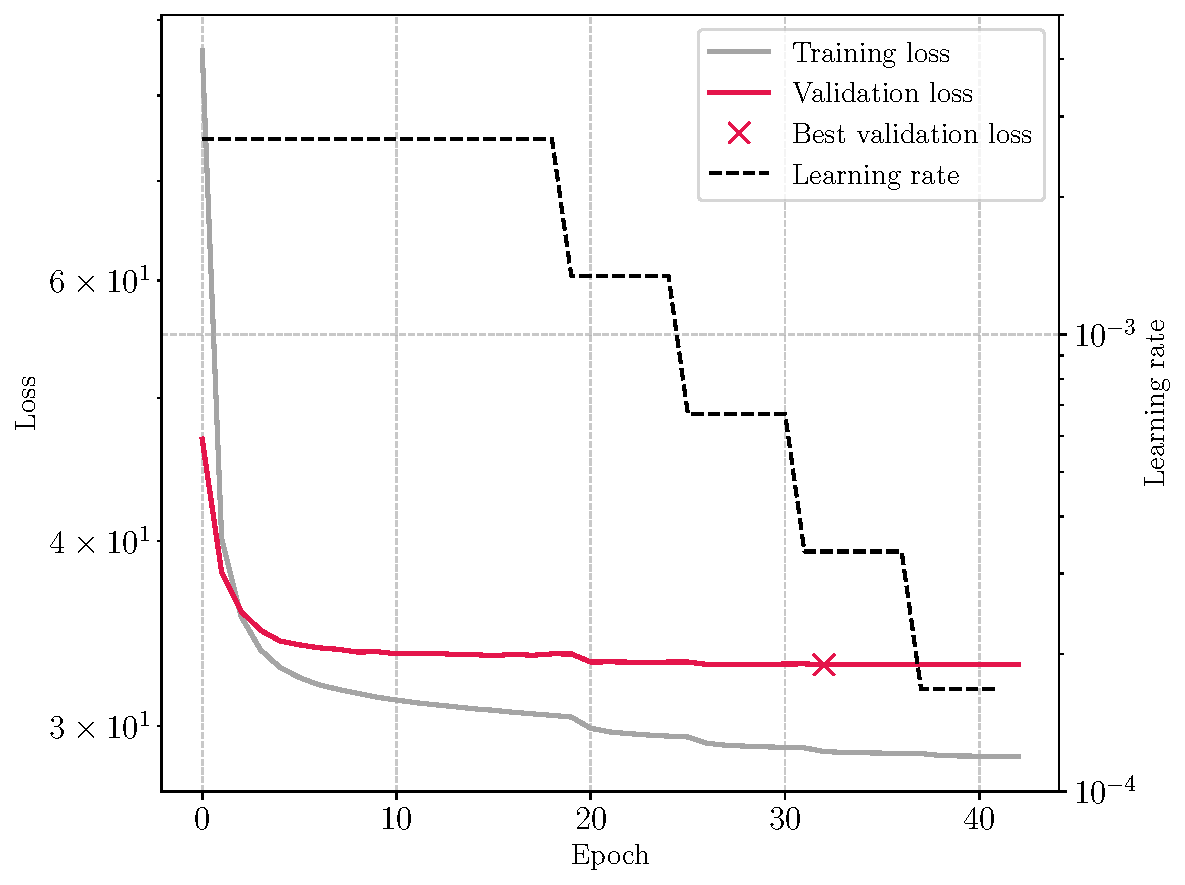
\includegraphics[width=\textwidth]{../fig/gnn/mgnn_pcseg1_simple_loss.pdf}
%     \caption[GNN initial training Loss]{\TODO{THIS IS A PLACEHOLDER!}}
%     \label{fig:gnn_initial_training_loss}
% \end{figure}